\documentclass[10pt]{beamer}


\geometry{paperwidth=160mm,paperheight=90mm}


\usepackage[T1]{fontenc}
\usepackage[utf8]{inputenc}
\usepackage{cabin} % font that is compatible with latex and inkscape. Not necassary when using xelatex  and one of your system fonts

\usepackage{tikz}
\usetikzlibrary{patterns}

\beamertemplatenavigationsymbolsempty

\tikzset{
    invisible/.style={opacity=0,text opacity=0},
    visible on/.style={alt=#1{}{invisible}},
    alt/.code args={<#1>#2#3}{%
      \alt<#1>{\pgfkeysalso{#2}}{\pgfkeysalso{#3}} 
    },
}


\begin{document}

\frame[plain]{
\visible<10>{
\begin{flushright}
\huge{\#sockit}
\end{flushright}}

\begin{center}
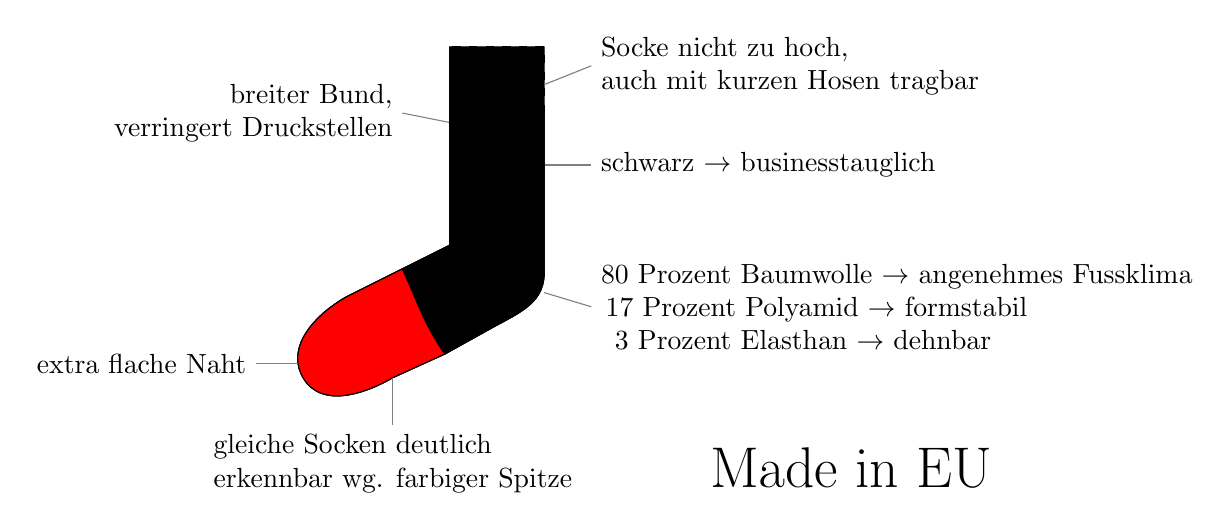
\begin{tikzpicture}[scale=0.60]

\coordinate (backleg) at (2,-0);
\coordinate (frontleg) at (0,-0);
\coordinate (instep) at (0,-2.8);
\coordinate (upperfoot) at (-1,-3.3);
\coordinate (uppertoes) at (-2.2,-3.9);
\coordinate (toetip) at (-3.1,-5.6);
\coordinate (soletoes) at (-1.2,-5.6);
\coordinate (sole) at (-0.1,-5.1);
\coordinate (soleheel) at (0.8,-4.6);
\coordinate (heel) at (2,-3.4);

\draw [fill=black,visible on = <1-2>] % long sock
([yshift=14mm]backleg)  --
	([yshift=14mm]frontleg) --(instep) --(upperfoot) -- (uppertoes) to [ out=210, in=120] (toetip) to [out=300, in=210] (soletoes) --
	(sole) -- (soleheel) to[out=30,in=270] (heel) -- cycle;

\draw[draw=gray, visible on = <2->] ([xshift=0mm, yshift=-11mm]backleg) -- ([xshift=1cm,yshift=-11mm]backleg) node[anchor=west,align=left] {
schwarz $\rightarrow$ businesstauglich};

\draw [fill = black, visible on = <3-5>] % short sock
(backleg)  --
	(frontleg) --(instep) --(upperfoot) -- (uppertoes) to [ out=210, in=120] (toetip) to [out=300, in=210] (soletoes) --
	(sole) -- (soleheel) to[out=30,in=270] (heel) -- cycle;

\draw [dashed, visible on = <3->] % shorten sock
(backleg)--([yshift=14mm]backleg) -- ([yshift=14mm]frontleg)--
	(frontleg);


\draw[draw=gray, visible on = <3->] ([xshift=0mm, yshift=6mm]backleg) -- ([xshift=10mm,yshift=10mm]backleg) node[anchor=west,align=left] {Socke nicht zu hoch,\\ auch mit kurzen Hosen tragbar}; %black

\draw[draw=gray, visible on = <4->] ([xshift=0mm, yshift=-2mm]frontleg) -- ([xshift=-1cm,yshift=0mm]frontleg) node[anchor=east,align=right] {breiter Bund,\\ verringert Druckstellen}; % wide  hem


\draw [draw=black,fill=black,visible on=<5->] % black fill
(backleg)  --
	(frontleg) --(instep) --(upperfoot) to[out=295,in=125]
	(sole) -- (soleheel) to[out=30,in=270] (heel) -- cycle;
	
\draw [draw=black,fill=red,visible on=<5->]
(sole) to[out=125,in=295]  (upperfoot) -- (uppertoes) to[out=210,in=120] (toetip) to[out=300,in=210] (soletoes) -- cycle; %red fill


\draw[draw=gray, visible on = <5->] ([xshift=0mm, yshift=0mm]soletoes) -- ([xshift=0cm,yshift=-1cm]soletoes) node[anchor=north,align=left] {gleiche Socken deutlich\\ erkennbar wg. farbiger Spitze};

\draw[draw=gray, visible on = <6->] ([xshift=-1mm, yshift=3mm]toetip) -- ([xshift=-1cm,yshift=3mm]toetip) node[anchor=east] {extra flache Naht};


\draw[draw=gray, visible on = <7->] ([xshift=0mm, yshift=-4mm]heel) -- ([xshift=1cm,yshift=-7mm]heel) node[anchor=west,align=left] {
80 Prozent Baumwolle $\rightarrow$ angenehmes Fussklima\\
\,17 Prozent Polyamid $\rightarrow$ formstabil\\
\,~3 Prozent Elasthan $\rightarrow$ dehnbar};


\node [visible on = <9-> ] at (8.5,-7.5)  {\huge{Made in EU}};

\end{tikzpicture}
\end{center}
}

\frame{
\pause
\vspace{18mm}
\begin{center}
\hspace{20mm}\huge{https://www.sockenpaket.de}
\end{center}
\pause % repeat frame multiple times 
\pause
\pause
}

\end{document} 
